\pdfbookmark{Общая характеристика работы}{characteristic}             % Закладка pdf
\section*{Общая характеристика работы}

\newcommand{\actuality}{\pdfbookmark[1]{Актуальность}{actuality}\underline{\textbf{\actualityTXT}}}
\newcommand{\progress}{\pdfbookmark[1]{Разработанность темы}{progress}\underline{\textbf{\progressTXT}}}
\newcommand{\aim}{\pdfbookmark[1]{Цели}{aim}\underline{{\textbf\aimTXT}}}
\newcommand{\tasks}{\pdfbookmark[1]{Задачи}{tasks}\underline{\textbf{\tasksTXT}}}
\newcommand{\aimtasks}{\pdfbookmark[1]{Цели и задачи}{aimtasks}\aimtasksTXT}
\newcommand{\novelty}{\pdfbookmark[1]{Научная новизна}{novelty}\underline{\textbf{\noveltyTXT}}}
\newcommand{\influence}{\pdfbookmark[1]{Практическая значимость}{influence}\underline{\textbf{\influenceTXT}}}
\newcommand{\methods}{\pdfbookmark[1]{Методология и методы исследования}{methods}\underline{\textbf{\methodsTXT}}}
\newcommand{\defpositions}{\pdfbookmark[1]{Положения, выносимые на защиту}{defpositions}\underline{\textbf{\defpositionsTXT}}}
\newcommand{\reliability}{\pdfbookmark[1]{Достоверность}{reliability}\underline{\textbf{\reliabilityTXT}}}
\newcommand{\probation}{\pdfbookmark[1]{Апробация}{probation}\underline{\textbf{\probationTXT}}}
\newcommand{\contribution}{\pdfbookmark[1]{Личный вклад}{contribution}\underline{\textbf{\contributionTXT}}}
\newcommand{\publications}{\pdfbookmark[1]{Публикации}{publications}\underline{\textbf{\publicationsTXT}}}


{\actuality}
К важнейшим проблемам XXI века относится решение задачи прогноза изменения климата, в значительной мере обусловленное антропогенным воздействием,
связанным с выбросами в атмосферу парниковых газов и других загрязняющих веществ, это можно наглядно увидеть в многочисленных отчетах
IPCC (Intergovernmental Panel on Climate Change) \optcite{IPCC21}.
Одним из основных современных инструментариев исследования изменчивости климата, понимания его прошлых изменений и прогнозирования будущих являются модели земной системы (МЗС),
главными компонентами которой являются модели общей циркуляции атмосферы и океана.
При этом в силу своих пространственных масштабов и физических свойств атмосфера служит «генератором» изменений климата,
а океан – основным «накопителем» этих изменений. Кроме того, океан в своем взаимодействии с атмосферой отвечает за генерацию десятилетних
и мультидесятилетних колебаний климата.
Поэтому создание вычислительно эффективной модели общей циркуляции океана (МОЦО), воспроизводящей сложную гидротермодинамику
Мирового океана является крайне важной задачей. Кроме того, создание эффективной модели морской гидротермодинамики на основе современных достижений
численного моделирования важно и для изучения физических процессов, формирующих региональную циркуляцию морей и океанов, что,
в свою очередь, необходимо для потребностей судоходства, рыболовства, оперативной океанографии и другие.

Современное интенсивное развитие климатических моделей и, в частности МОЦО, в настоящее время связано в первую очередь с бурным развитием вычислительной техники.
Появление терафлопных и петафлопных вычислительных систем, т.н. суперкомпьютеров, открыло возможности для построения глобальных моделей с
высоким пространственным разрешением, которые позволяют описывать мезо- и субмезо масштабы вихревой изменчивости океана и проводить с ними расчеты на долгие сроки.
На сегодняшний день большинство высокопроизводительных вычислительных систем являются гетерогенными, объединяющими различные типы вычислительных процессоров.
Это можно наглядно увидеть из списка TOP 500 самых мощных суперкомпьютеров в мире \optcite{TOP500}.
Такие системы в общем случае могут состоять из большого количества процессоров разного типа.
В наши дни выделяют основное направление развития гетерогенных систем, состоящее в совместном использовании многоядерного центрального процессора (CPU)
и массивно-параллельных ускорителей, например графических процессоров (GPU).
Суперкомпьютерная техника стремительно развивается в России и тенденция развития схожа с мировой - это можно видеть из списка ТОП 50
самых мощных суперкомпьютеров в СНГ \optcite{TOP50}.
Мощнейший суперкомпьютер России «Ломоносов-2» в МГУ им. М.В.Ломоносова являются вычислительной системой именно гетерогенного типа \optcite{L2}.
Создание модели гидродинамики океана, использующую эффективно ресурсы таких гетерогенных вычислительных систем,
является сложной и актуальной на сегодняшний день задачей.

Основной целью настоящего проекта является усовершенствование российской сигма-модели общей циркуляции океана INMOM
(Institute of Numerical Mathematics Ocean Model) для эффективного использования на массивно-параллельных и гетерогенных вычислительных системах \optcite{INMOM}.
Модель INMOM разрабатывается в ИВМ РАН (Институт вычислительной математики РАН) и уже на протяжении более полутора десятков лет используется
в качестве океанического блока МЗС INMCM (Institute of Numerical Mathematic Climate Model) различных версий \optcite{VolodinINMCM2013}.
Именно эта совместная модель является пока единственным представителем от России в различных этапах международного проекта сравнения климатических моделей CMIP (Coupled Model Intercomparison Project), проводящегося под эгидой IPCC (International Panel on Climate Change, или в русской транскрипции МГЭИК – Межправительственная группа экспертов по изменению климата).
Последнее такое сравнение CMIP6 (CMIP, Phase 6) включено в шестой отчет IPCC, недавно проходившего в 2010-2013 гг. под эгидой IPCC (International Panel on Climate Change,
или в русской транскрипции МГЭИК – Межправительственная группа экспертов по изменению климата).
Модель написана на языке Fortran 90/95.

Следует особо подчеркнуть оригинальность как сигма-модели общей циркуляции океана INMOM, так и самой модели климата INMCM, разработанных в ИВМ РАН.
Возникающий при этом в рамках CMIP «параллелизм» необходим для контроля воспроизводимости получаемых результатов и для статистического исключения возможных
ошибок прогноза изменений климата. Это особо ценится в проекте CMIP, т.к. позволяет учитывать больший спектр климатической изменчивости.
Именно для этого проводилось и проводится сравнение результатов моделирования климата и его изменений с помощью различных МЗС в рамках международных программ,
являющиеся клубами высоких технологий. С этой точки зрения следует особо подчеркнуть,
что INMOM - это единственная сигма–координатная модель, способная адекватно воспроизводить климатическую циркуляцию Мирового океана при расчетах на большие времена.

%Модель относится к классу сигма-моделей океана:
%в ней в качестве вертикальной переменной используется безразмерная величина $\sigma \in [0, 1]$, которая определяется из соотношения:
%$$ \sigma = \frac{z + \zeta}{H + \zeta} $$
%где $z$ - направленная вниз обычная вертикальная координата по глубине, с началом на невозмущенной поверхности океана;
%$\zeta$ - отклонение уровня океана от невозмущенной поверхности; 
%$H$ - глубина океана в состоянии покоя.
%Модель написана на языке Fortran 90/95.
%Предыдущая версия модели INMOM используется в качестве океанического блока 
%климатической модели INMCM (Institute of Numerical Mathematics Climate Model), созданной в ИВМ РАН и участвующей в программе
%IPCC по прогнозированию изменений климата \optcite{VolodinINMCM2013}.

В работе отдельно рассматривается система нелинейных уравнений мелкой воды,
являющаяся блоком сигма-модели общей циркуляции океана INMОM.
Система уравнений мелкой воды является неотъемлемой и одной из самых важных подзадач в моделях общей циркуляции океана \optcite{ROMS2005}, \optcite{Ibraev2015}.
Решение этой системы уравнений занимает существенную часть времени, необходимого для решения полной задачи циркуляции океана,
как было показано, например, в работе \cite{ChaplyginINMOM2017}.
Кроме того, на основе нелинейных уравнений мелкой воды реализуются наиболее продвинутые системы
предупреждения о цунами \optcite{TUNAMI}, реализованные для Мирового океана с высоким пространственным разрешением.
Поэтому возникает вопрос об эффективной параллельной реализации алгоритма решения системы уравнений мелкой воды.

Следует особо подчеркнуть необходимость развития суперкомпьютерных технологий в России и развития отечественных моделей, поскольку это является необходимым условием обеспечения независимой экспертизы формирования климатических изменений и изменчивости циркуляции Мирового океана как в глобальном, так и на региональном масштабах.
%что, в свою очередь, является необходимым условием национальной безопасности России.

% {\progress}
% Этот раздел должен быть отдельным структурным элементом по
% ГОСТ, но он, как правило, включается в описание актуальности
% темы. Нужен он отдельным структурынм элемементом или нет ---
% смотрите другие диссертации вашего совета, скорее всего не нужен.

{\aim} данной работы является разработка усовершенствованной версии сигма-модели общей циркуляции океана INMOM и модели мелкой воды для эффективного использования на массивно-параллельных многопроцессорных и гетерогенных вычислительных системах.

%Целью настоящего проекта является исследовать эффективность работы усовершенствованной версии INMOM на разных типах вычислительных систем, провести анализ масштабируемости и производительности. Провести численные эксперименты с этой моделью по воспроизведению циркуляции океана с вихредопускающим и вихреразрешающим пространственным разрешением около 25 и 10 км соответственно.
%Подготовить усовершенствованную версию INMOM к включению в качестве нового океанического блока в МЗС INMCM.
%Планируемые эксперименты с моделью INMOM позволят также продвинутся в ее дальнейшем улучшении.
%Следует особо подчеркнуть необходимость развития суперкомпьютерных технологий в России и развития отечественных моделей,
%поскольку это является необходимым условием обеспечения независимой экспертизы формирования климатических изменений и изменчивости циркуляции
%Мирового океана как в глобальном, так и на региональном масштабах, что, в свою очередь, является необходимым условием национальной безопасности России.

Для~достижения поставленной цели необходимо было решить следующие {\tasks}:
\begin{enumerate}[beginpenalty=10000] % https://tex.stackexchange.com/a/476052/104425
    \item Разработать программную архитектуру сигма-модели общей циркуляции океана INMOM и, в частности, модели мелкой воды, предполагающую гибкий переход на гибридные модели параллельного программирования с использованием технологий MPI, OpenMP, CUDA.
    \item Разработать параллельные вычислительные алгоритмы решения нелинейных уравнений мелкой воды для использования на массивно-параллельных многопроцессорных и гетерогенных вычислительных системах.
    \item Разработать метод балансировки нагрузки вычислений на процессорах для улучшения масштабируемости и производительности моделей на высокопроизводительных вычислительных системах.
    \item На основе разработанных параллельных вычислительных алгоритмов решения нелинейных уравнений мелкой воды разработать усовершенствованную версию сигма-модели общей циркуляции океана INMOM для эффективного использования на массивно-параллельных многопроцессорных вычислительных системах.
    \item Исследовать масштабируемость и производительность предложенных методов на массивно-параллельных и гетерогенных вычислительных системах. 
%\item Разработать гибридные модели параллельного программирования для эффективного использования на массивно-параллельных многопроцессорных  и гетерогенных вычислительных системах.
\end{enumerate}

%1. Создание эффективной параллельной реализации уравнений мелкой воды, которые являются одним из основных блоков INMOM. Система уравнений мелкой воды является неотъемлемой и одной из самых важных подзадач не только в INMOM, но и в любой другой МОЦО. Решение этой системы уравнений занимает существенную часть времени, необходимого для решения полной задачи циркуляции океана. Кроме того, на основе нелинейных уравнений мелкой воды реализуются наиболее продвинутые системы предупреждения о цунами, реализованные для Мирового океана с высоким пространственным разрешением. Поэтому вопрос об эффективной параллельной реализации алгоритма решения системы уравнений мелкой воды особенно актуален.
%2. Создание эффективной параллельной реализации всех блоков INMOM. При построении усовершенствованной модели циркуляции океана за основу будут взяты параллельные методы и подходы, применяемые в модели мелкой воды из предыдущей задачи. Обобщение таких методов и подходов от двумерного случая мелкой воды к трехмерной задаче циркуляции океана будет происходить без существенных изменений и сложностей, т.к. модель океана INMOM является сигма-моделью с одинаковым числом расчетных уровней по глубине для всех точек сетки по горизонтали.
%3. Тестирование усовершенствованной модели циркуляции океана INMOM на различных массивно-параллельных и гетерогенных вычислительных системах. В качестве основных платформ для тестирования планируется использовать суперкомпьютеры «Ломоносов» и «Ломоносов-2», а также суперкомпьютеры ИВМ РАН и МСЦ РАН. Будет проведен комплексный анализ масштабируемости и производительности усовершенствованной модели океана на различных вычислительных системах.
%4. Проведение численных экспериментов по воспроизведению циркуляции океана с использованием усовершенствованной модели INMOM. Для этого будет реализована версии INMOM для акватории Мирового океана с вихредопускающим пространственным разрешением, а для Атлантического океана и с вихреразрешающим разрешением. Будет проведен комплексный анализ полученных результатов, которые позволят продвинуться как в дальнейшем улучшении эффективности модели, так и в решении ряда практических и научных задач.
%5. Подготовка усовершенствованной версии INMOM к включению в качестве нового океанического блока в МЗС INMCM. Для каждой совместной модели задача интерполяции данных между сетками является крайне важной. Поэтому в рамках этой задачи будет предложен и реализован эффективный параллельный алгоритм интерполяции для произвольных пар прямоугольных сеток.

{\novelty}
\begin{enumerate}[beginpenalty=10000] % https://tex.stackexchange.com/a/476052/104425
    \item Разработаны параллельные алгоритмы решения нелинейных уравнений мелкой воды для эффективного использования на массивно-параллельных и гетерогенных вычислительных системах, представленные в виде отдельного программного комплекса. Этот программный комплекс можно использовать как в качестве блока сигма-модели циркуляции океана INMOM, так и независимо.
    \item Разработана усовершенствованная версия российской сигмы-модели общей циркуляции океана INMOM для эффективного использования на массивно-параллельных многопроцессорных вычислительных системах.
    \item Разработан метод балансировки нагрузки вычислений на процессорах для улучшения масштабируемости и производительности сигмы-модели общей циркуляции океана INMOM на высокопроизводительных вычислительных системах.
\end{enumerate}

{\influence}
Разработанный программный комплекс решения нелинейных уравнений воды можно использовать как в качестве блока сигма-модели циркуляции океана INMOM, так и независимо, например для расчетов прохождения волны цунами, штормов, приливов и ветрового нагона. С помощью разработанного программного комплекса проводилось моделирование цунами в Японии и экстремального шторма на Азовском море, было показано, что результаты вычислений согласуются с данными наблюдений.
Разработанная усовершенствованная сигма-модель общей циркуляции океана INMOM может эффективно использоваться на массивно-параллельных многопроцессорных вычислительных системах, что позволяет существенно сократить время расчетов без ухудшения точности результатов. Эффективность параллельной реализации подтверждена тестами на современных российских суперкомьютерах. На основе усовершенствованной сигма-модели океана INMOM была построена система оперативного моделирования Северного Ледовитого океана и прилегающих к нему акваторий (INMOM-Арктика). Результаты сравнения расчетов и данных наблюдений свидетельствуют, что модель INMOM-Арктика позволяет корректно воспроизводить циркуляцию Северного Ледовитого океана.
Предполагается, что усовершенствованная версия сигма-модели океана INMOM будет использована в качестве нового океанического блока в МЗС INMCM.

{\methods}
Теория и методы вычислительной математики; численные эксперименты на современных суперкомпьютерах; современные инструменты для разработки, отладки и профилирования программного комплекса на распределенных и гетерогенных вычислительных системах.

{\defpositions}
\begin{enumerate}[beginpenalty=10000] % https://tex.stackexchange.com/a/476052/104425
    \item Разработана программная архитектура сигма-модели общей циркуляции океана INMOM и, в частности, модели мелкой воды, предполагающая гибкий переход на гибридные модели параллельного программирования с использованием технологий MPI, OpenMP, CUDA.    
    \item Разработаны параллельные вычислительные алгоритмы решения нелинейных уравнений мелкой воды для использования на массивно-параллельных многопроцессорных и гетерогенных вычислительных системах.
    \item Разработан метод балансировки нагрузки вычислений на процессорах для улучшения масштабируемости и производительности моделей на высокопроизводительных вычислительных системах.
    \item На основе разработанных параллельных вычислительных алгоритмов решения нелинейных уравнений мелкой воды разработана усовершенствованная версия сигма-модель общей циркуляции океана INMOM для эффективного использования на массивно-параллельных многопроцессорных вычислительных системах.
    \item Исследована масштабируемость и производительность предложенных методов на массивно-параллельных и гетерогенных вычислительных системах.     
%\item Разработаны гибридные модели параллельного программирования для эффективного использования на массивно-параллельных многопроцессорных и гетерогенных вычислительных системах.
\end{enumerate}
%В папке Documents можно ознакомиться с решением совета из Томского~ГУ
%(в~файле \verb+Def_positions.pdf+), где обоснованно даются рекомендации
%по~формулировкам защищаемых положений.

{\reliability} полученных результатов обеспечивается использованием в работе теории численных методов, а также сравнением результатов вычислительных экспериментов с данными наблюдений. Материал, изложенный в диссертации, опирается на широкий список научной литературы, посвящённый рассматриваемым методам.

{\probation}
Основные результаты работы докладывались~на:
\begin{enumerate}[beginpenalty=10000]
\item Конференции "Труды 60-й Всероссийской научной конференции МФТИ" (г. Москва, 2017).
\item Конференции "Труды VI международной научно-практической конференции Морские исследования и образование: MARESEDU-2017" (2017).
\item Международной конференции "EGU 2019" (2019).
\item Семинаре "Новые подходы к измерениям и моделированию геофизической турбулентности" (г. Москва, НИВЦ МГУ, 2019).
\item Международной конференции "Математическое моделирование и суперкомпьютерные технологии" (г. Нижний Новгород, 2020).
\end{enumerate}

{\contribution} Автором лично разработаны параллельные алгоритмы решения нелинейных уравнений мелкой воды для эффективного использования на массивно-параллельных и гетерогенных вычислительных системах и разработана усовершенствованная версия российской сигма-модели общей циркуляции океана INMOM для эффективного использования на массивно-параллельных многопроцессорных вычислительных системах. Представленная диссертация является самостоятельным законченным трудом автора. 

{\publications}
Основные результаты по теме диссертации изложены
в~7~печатных изданиях: \cite{ChaplyginINMOM2017}, \cite{ChaplyginSW2017}, \cite{ChaplyginAzov2017},\cite{DianskyInertOsc2019}, \cite{ChaplyginLB2019}, \cite{ChaplyginSW2021}, \cite{Chaplygin_Gusev_Diansky_2022}, 
5 из которых изданы в журналах, рекомендованных ВАК, 2 индексируются в международных базах данных Scopus или Web of Science.
 % Характеристика работы по структуре во введении и в автореферате не отличается (ГОСТ Р 7.0.11, пункты 5.3.1 и 9.2.1), потому её загружаем из одного и того же внешнего файла, предварительно задав форму выделения некоторым параметрам

Диссертационная работа была выполнена при поддержке гранта РФФИ № 20-31-90109.

%\underline{\textbf{Объем и структура работы.}} Диссертация состоит из~введения,
%четырех глав, заключения и~приложения. Полный объем диссертации
%\textbf{ХХХ}~страниц текста с~\textbf{ХХ}~рисунками и~5~таблицами. Список
%литературы содержит \textbf{ХХX}~наименование.

\pdfbookmark{Содержание работы}{description}                          % Закладка pdf
\section*{Содержание работы}
Во \underline{\textbf{введении}} обосновывается актуальность
исследований, проводимых в~рамках данной диссертационной работы,
%приводится обзор научной литературы по~изучаемой проблеме,
формулируется цель, ставятся задачи работы, излагается научная новизна
и практическая значимость представляемой работы.

%В~последующих главах сначала описывается общий принцип, позволяющий \dots, а~потом идёт апробация на частных примерах: \dots  и~\dots.

\underline{\textbf{Первая глава}} посвящена математической формулировки задачи моделирования общей циркуляции океана и особенностям численной реализации сигма-модели общей циркуляции океана INMOM.

В \underline{\textit{разделе 1.1}} представлена математическая формулировка задачи моделирования общей циркуляции океана, основанной на системе уравнений гидротермодинамики в приближениях гидростатики и Буссинеска для сферического слоя на Земле в предположении ее постоянного радиуса.
В разделе представлено описание перехода системы уравнений гидротермодинамики океана в новую систему координат с использованием вертикальной координаты $\sigma$, используемой в модели общей циркуляции океана INMOM.
Сигма координата зависит от горизонтальных координат, отклонения уровня и глубины океана, и в главе представлен подробный анализ трудностей и особенностей применения сигма-моделей океана, включая погрешности в аппроксимации горизонтального градиента давления. Описаны методы снижения этих погрешностей, учитывая особенности разностной аппроксимации градиентов давления.
%Подробное описание численной реализации модели включает в себя специфику пространственной аппроксимации на 'C'-сетке и методику построения согласованных операторов разностной аппроксимации. Описанная схема по времени позволяет эффективно решать систему уравнений гидротермодинамики океана на каждом шаге интегрирования.
Данный раздел также включает описание подготовки к решению системы уравнений гидротермодинамики океана, включая приведение к дивергентному виду и симметризацию градиента давления. 

В \underline{\textit{разделе 1.2}} представлено подробное описание численной реализации модели, включая специфику пространственной аппроксимации на 'C'-сетке по классификации Аракавы и методику построения согласованных операторов разностной аппроксимации.
В разделе описывается двухслойная схема по времени, которая используется для интегрирования модели. Процесс интегрирования включает линеаризацию нелинейных слагаемых, что позволяет рассчитывать переменные на новом временном шаге, исходя из значений на предыдущем шаге.
Описанная схема по времени позволяет эффективно решать систему уравнений гидротермодинамики океана на каждом шаге интегрирования.
%Представляет пространственно аппроксимации модели, которая базируется на 'C'-сетке по классификации Аракавы. Эта сетка является нерегулярной по долготе и широте, а также неравномерной по вертикали. Для численного решения системы уравнений гидротермодинамики океана применяется разностная аппроксимация второго порядка точности. Особое внимание уделяется сохранению свойств симметрии разностных аналогов операторов, соблюдая их энергетические соотношения.
%Кроме того, описывается двухслойная схема по времени, которая используется для интегрирования модели. Процесс интегрирования включает линеаризацию нелинейных слагаемых, что позволяет рассчитывать переменные на новом временном шаге, исходя из значений на предыдущем шаге.

В \underline{\textit{разделе 1.3}} описывается общая схема численного решения системы уравнений гидротермодинамики океана с использованием метода расщепления Г.И. Марчука. Метод основан на физическом расщеплении процессов и включает инициализацию, основной цикл по времени и финализацию.
%Основной цикл включает определение текущего модельного времени, задание потоков на поверхности и открытых границах, расчет компонентов напряжений, коэффициентов турбулентного обмена, углов наклона для универсальной диффузии, расчет потоков на поверхности и дне, а также обновление толщины океана и вертикальной скорости в соответствии с уравнением неразрывности.
%Также осуществляется расчет коэффициентов вертикального обмена с использованием различных параметризаций, анализ температуры и солености с учетом различных схем переноса, диффузии для компонентов скорости, а также расчет плотности по обновленным значениям температуры и солености.
%Процедуры бароклинной и баротропной адаптации способствуют эффективной стабилизации расчетов по скорости внутренних волн и внешних гравитационных волн соответственно.
%Глава завершается описанием инструмента для решения систем линейных алгебраических уравнений, используемого для решения системы уравнений мелкой воды. Предложенный алгоритм успешно применяется для динамических расчетов океана и повторяется до достижения заданного расчетного времени."

\underline{\textit{Раздел 1.4}} описывает систему оперативного моделирования Северного Ледовитого океана и прилегающим к нему акваторий (INMOM-Арктика) построенную на основе усовершенствованной сигма-модели общей циркуляции океана INMOM.
Результаты сравнения расчетов и данных наблюдений свидетельствуют, что модель INMOM-Арктика с использованием предложенных условий на открытых границах позволяет корректно воспроизводить циркуляцию Северного Ледовитого океана.

В завершении, в \underline{\textit{разделе 1.5}} приводятся результаты анализа данных численного моделирования циркуляции Черного моря в период шторма, их физическая интерпретация, а также исследование аналитического решения описывающей их системы уравнений.

\underline{\textbf{Вторая глава}} посвящена математической постановке задачи модели мелкой воды как составной части модели гидродинамики океана и численной реализации решения системы уравнений мелкой воды, представленной в работе в виде отдельного программного комплекса.

В \underline{\textit{разделе 2.1}} рассматривается математическая постановка системы нелинейных уравнений мелкой воды в произвольной ортогональной системе координат, которая возникает при разрешении быстрых баротропных гравитационных волн в сигма-модели общей циркуляции океана INMOM.

\underline{\textit{Раздел 2.2}} посвящен описанию численной реализации модели мелкой воды, включая специфику использования методов дискретизации по пространству на 'C'-сетке по классификации Аракавы и специфику использования численной схемы 'Чехарда со средней точкой' для дискретизации по времени.

В \underline{\textit{разделе 2.3}} представлены результаты использования модели мелкой воды для моделирования цунами 2011 года в Японии и экстремального шторма на Азовском море в 2013 году. Важной частью исследования было сравнение результатов моделирования с экспериментальными данными и анализ различий в расчетах по нелинейным и линеаризованным уравнениям мелкой воды. Линеаризованные уравнения являются упрощением нелинейной системы, где используется предположение $h \approx H$ при условии $\zeta << H$.
Анализ указывает на хорошее соответствие результатов моделирования с данными наблюдений, и также было показано, что вклад нелинейности в контексте данных экстремальных событий незначителен.

\underline{\textbf{Третья глава}} посвящена описанию разработанных параллельных алгоритмов и особенностям параллельной реализации в модели мелкой воды и сигма-модели общей циркуляции океана INMOM.

\underline{\textit{Раздел 3.1}} представляет подробный анализ разработанной программной архитектуры модели мелкой воды и методов параллельных вычислений для эффективного использования модели на различных вычислительных системах.
Программная архитектура является ключевым элементом, определяющим гибкость, масштабируемость и переносимость модели на различные типы вычислительных систем. Представленная в работе архитектура базируется на принципе разделения обязанностей, что позволяет выделить три уровня программного комплекса: Ядро (содержит все вычислительные подпрограммы модели), Алгоритм (описывает основной временной цикл модели) и Интерфейс (реализует все параллельные методы и подходы в модели).
Этот подход значительно упрощает интеграцию новых компонентов и алгоритмов, а также облегчает адаптацию кода под различные вычислительные системы без изменений в основных вычислительных процедурах.

В \underline{\textit{разделе 3.2}} представлен усовершенствованный двумерный метод декомпозиции области, так называемый блочный подход, используемый в модели в качестве основного метода распараллеливания для вычислительных архитектур с распределенной памятью.
Рассматриваемый блочный подход позволяет формировать подобласти произвольной формы, обеспечивая балансировку нагрузки вычислений на процессоры, и эффективно использовать кэш-память.

В \underline{\textit{разделе 3.3}} описан метод балансировки нагрузки вычислений на процессоры с использованием фрактальной кривой Гильберта в двумерном пространстве.
Методы балансировки нагрузки вычислений позволяют снизить время простоя отдельных процессоров и тем самым повысить эффективность параллельной программы, что существенно важно при решении задач на высокопроизводительных вычислительных системах.
В данной главе показано, что предложенный метод балансировки нагрузки показывает хорошие результаты применительно к решению уравнений мелкой воды, а также показано сравнение этого метода с методом балансировки нагрузки, основанном на графах из библиотеки METIS.

В \underline{\textit{разделе 3.4}} и \underline{\textit{разделе 3.5}} представлены различные модели параллельного программирования для использования на многопроцессорных и гетерогенных вычислительных системах (см. рис. \ref{fig:patterns}):

\begin{enumerate}

\item Чистый MPI подход для использования на вычислительных архитектурах с распределенной памятью.
\item Гибридный MPI-OpenMP подход для использования на многопроцессорных систем с общей памя­тью.
\item Гибридный синхронный MPI-OpenMP-CUDA подход для использования на гетерогенных вычислительных системах.
\item Гибридный MPI-OpenMP-CUDA подход для использования на гетерогенных вычислительных системах с несколькими GPU на вычислительном узле.
\item Гибридный асинхронный MPI-CUDA подход для использования на гетерогенных вычислительных системах с перекрытием передачи данных и выполнения по времени.

\end{enumerate}

\begin{figure}[!ht]
	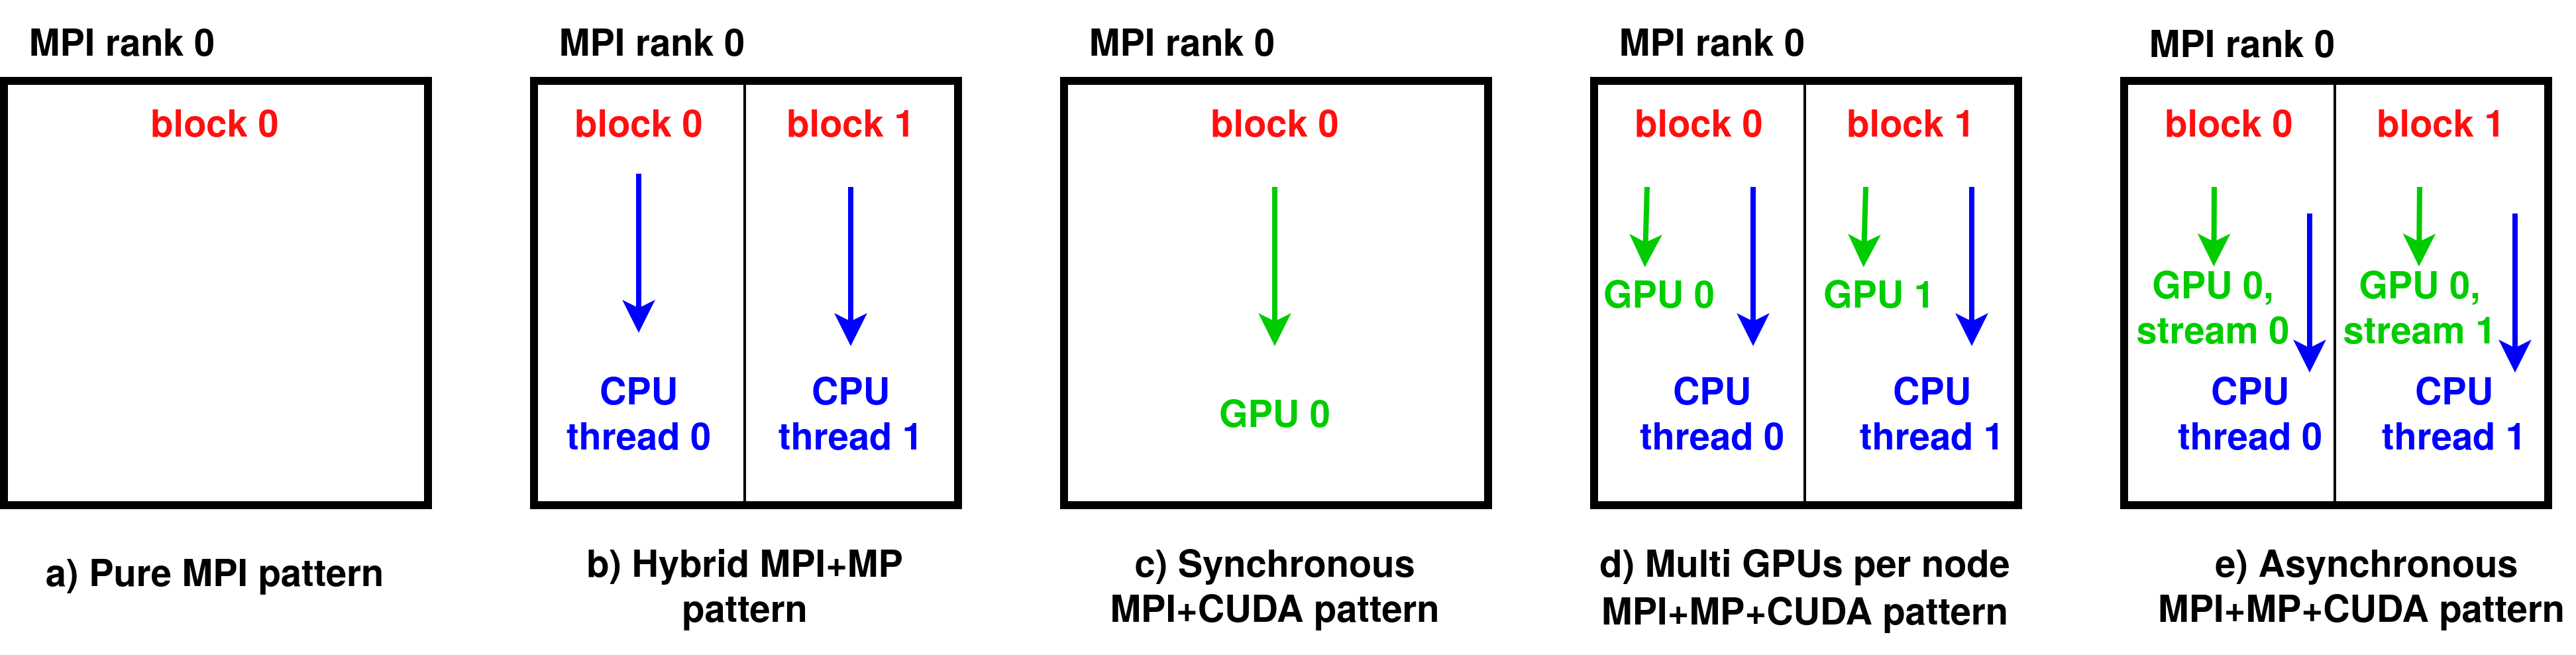
\includegraphics[width=\linewidth]{CPU_GPU_patterns.png}
	\vspace{3pt}
	\caption{Параллельные шаблоны программирования реализованные в модели}
	\label{fig:patterns}
\end{figure}

%5Можно сослаться на свои работы в автореферате. Для этого в файле \verb!Synopsis/setup.tex! необходимо присвоить положительное значение счётчику \verb!\setcounter{usefootcite}{1}!. В таком случае ссылки на работы других авторов будут подстрочными. Изложенные в третьей главе результаты опубликованы в~\cite{vakbib1, vakbib2}. Использование подстрочных ссылок внутри таблиц может вызывать проблемы.

В \underline{\textit{разделе 3.6}} приводится описание реализации усовершенствованной параллельной версии сигма-модели общей циркуляции океана INMOM, основанной на разработанных параллельных вычислительных алгоритмах решения нелинейных уравнений мелкой воды.
В сигма-модели океана INMOM были поддержаны гибридные модели параллельного программирования для использования на многопроцессорных вычислительных системах, подробно описанные в разделе 3.4.
Описаны усовершенствованный двумерный метод декомпозиции области (блочный подход) и особенности синхронизации внерасчетных границ применительно к трехмерной задаче.
В разделе описан метод баланси­ровки нагрузки вычислений с использованием кривых Гильберта применительно к трехмерным уравнением гидротермодинамики океана, используемых в модели INMOM.
Важно отметить, что оптимальность разбиения для мелкой воды точно соответствует оптимальности для трехмерной сигма-модели INMOM, так как количество расчетных уровней по глубине в модели одинаково для всех точек сетки по горизонтали.
Были также описаны детали реализации решателя системы алгебраических уравнений, возникающих в модели океана на этапе баратропной адаптации.

В \underline{\textbf{четвертой главе}} приведены результаты исследования производительности и масштабируемости моделей мелкой воды и общей циркуляции океана INMOM на современных суперкомпьюетрах.

В \underline{\textit{разделе 4.1}} приведены результаты исследования масштабируемости модели мелкой воды, проведенные на суперкомпьютере Ломоносов-2 в Мос­ковском государственном университете имени Ломоносова.
%Первая серия вычислительных экспериментов проводилась для акватории без участков суши. Эта серия экспериментов проводилась с целью продемон­стрировать производительность модели без эффектов неравномерной нагрузки на процессоры.
В разделе был проведён анализ эффективности и масштабируемости гибридных методов для расчётов мелкой воды с использованием GPU в сравнении с методами расчётов на CPU (см. рис \ref{fig:TheBox}). 
Продемонстрирована масштабируемость различных подходов на CPU и GPU для расчётных областей 1525 на 1115 и 6100 на 4460 точек: производительность на одну точку сетки на GPU резко снижается после $2^{19}$ точек на узел, в то время как производительность на CPU отлично масштабируется до $2^{17}$ точек (см. рис \ref{fig:TheBox_full}). Это связано с тем, что небольшой размер сетки не может в достаточной степени загрузить GPU и скрыть задержки при обращении к памяти. Кроме того, накладные расходы на передачу данных между CPU и GPU становятся значительными при небольших размерах сетки. Таким образом, получается снижение производительности GPU при небольших размерах сетки.  Тем не менее, вычисления на GPU превосходят вычисления на CPU в 4,7 раза на 30 узлах, использующих 360 ядер CPU и 60 GPU при размере сетки 6100 $\times$ 4460.  

\begin{figure}[!ht]
	\begin{minipage}{0.5\linewidth}
	\centering
	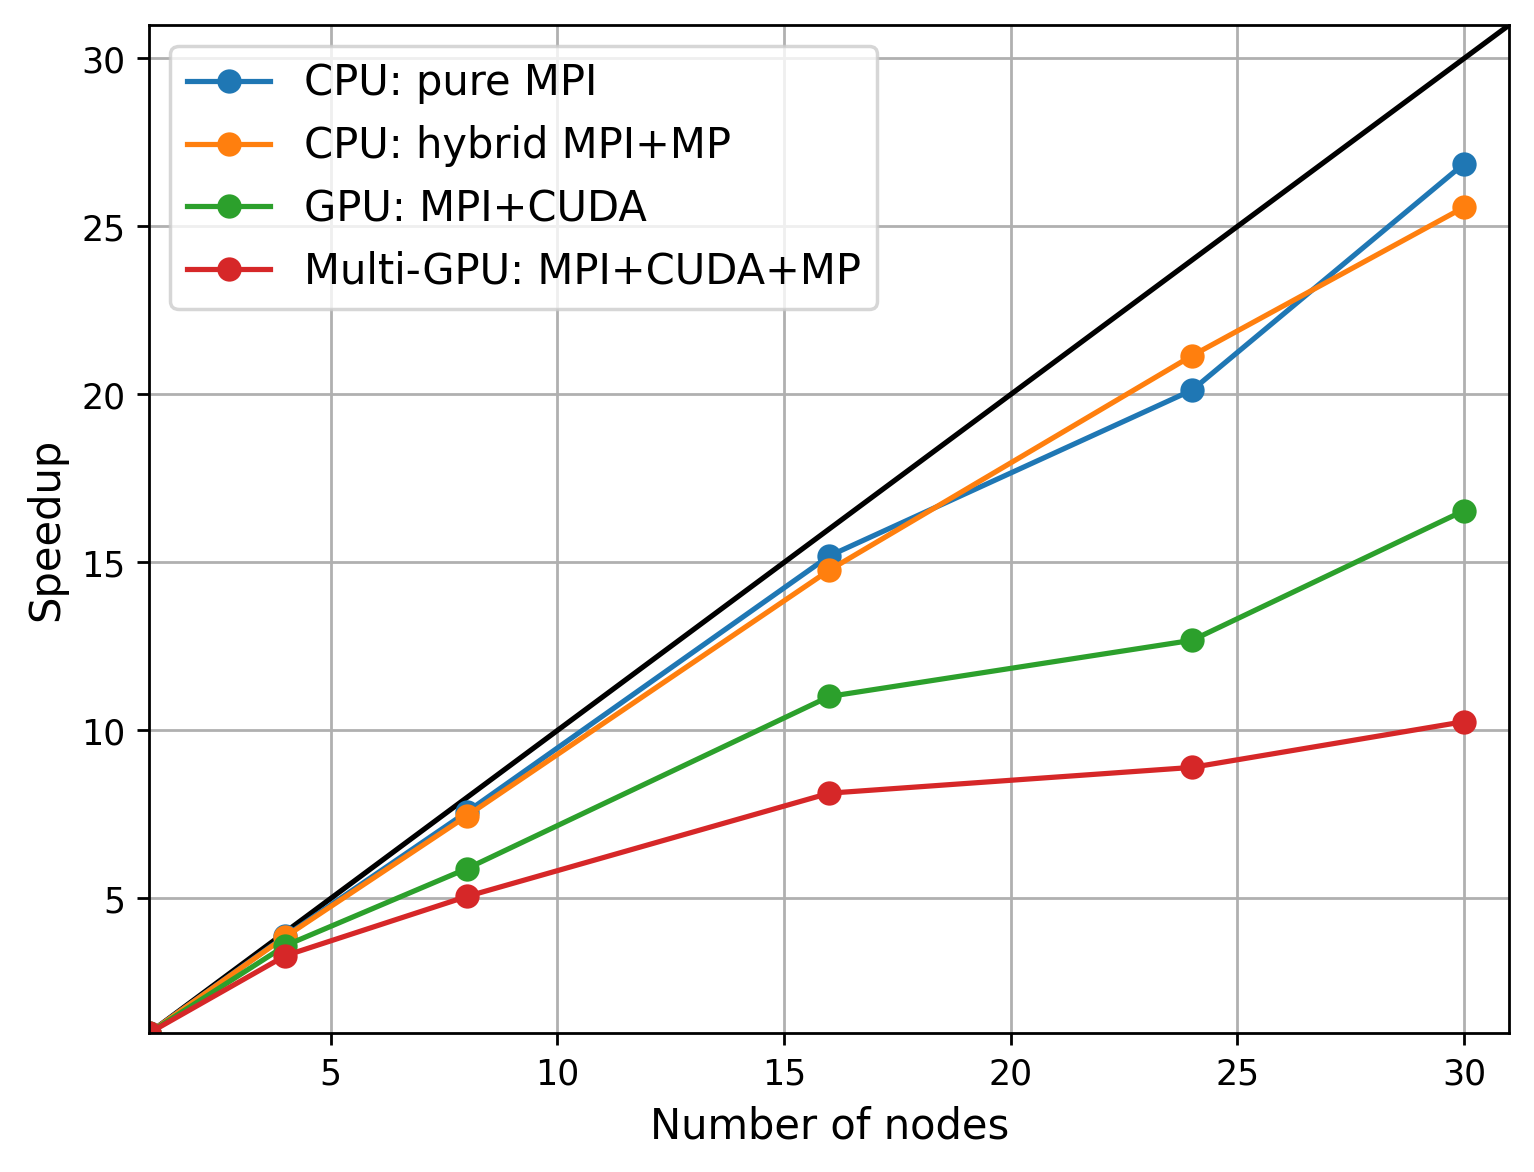
\includegraphics[width=\linewidth]{v3_3_6100x4460_pascal_speedup_multiGPU_V.png}
	\subcaption{Ускорение}
	\end{minipage}
	\begin{minipage}{0.5\linewidth}
	\centering
    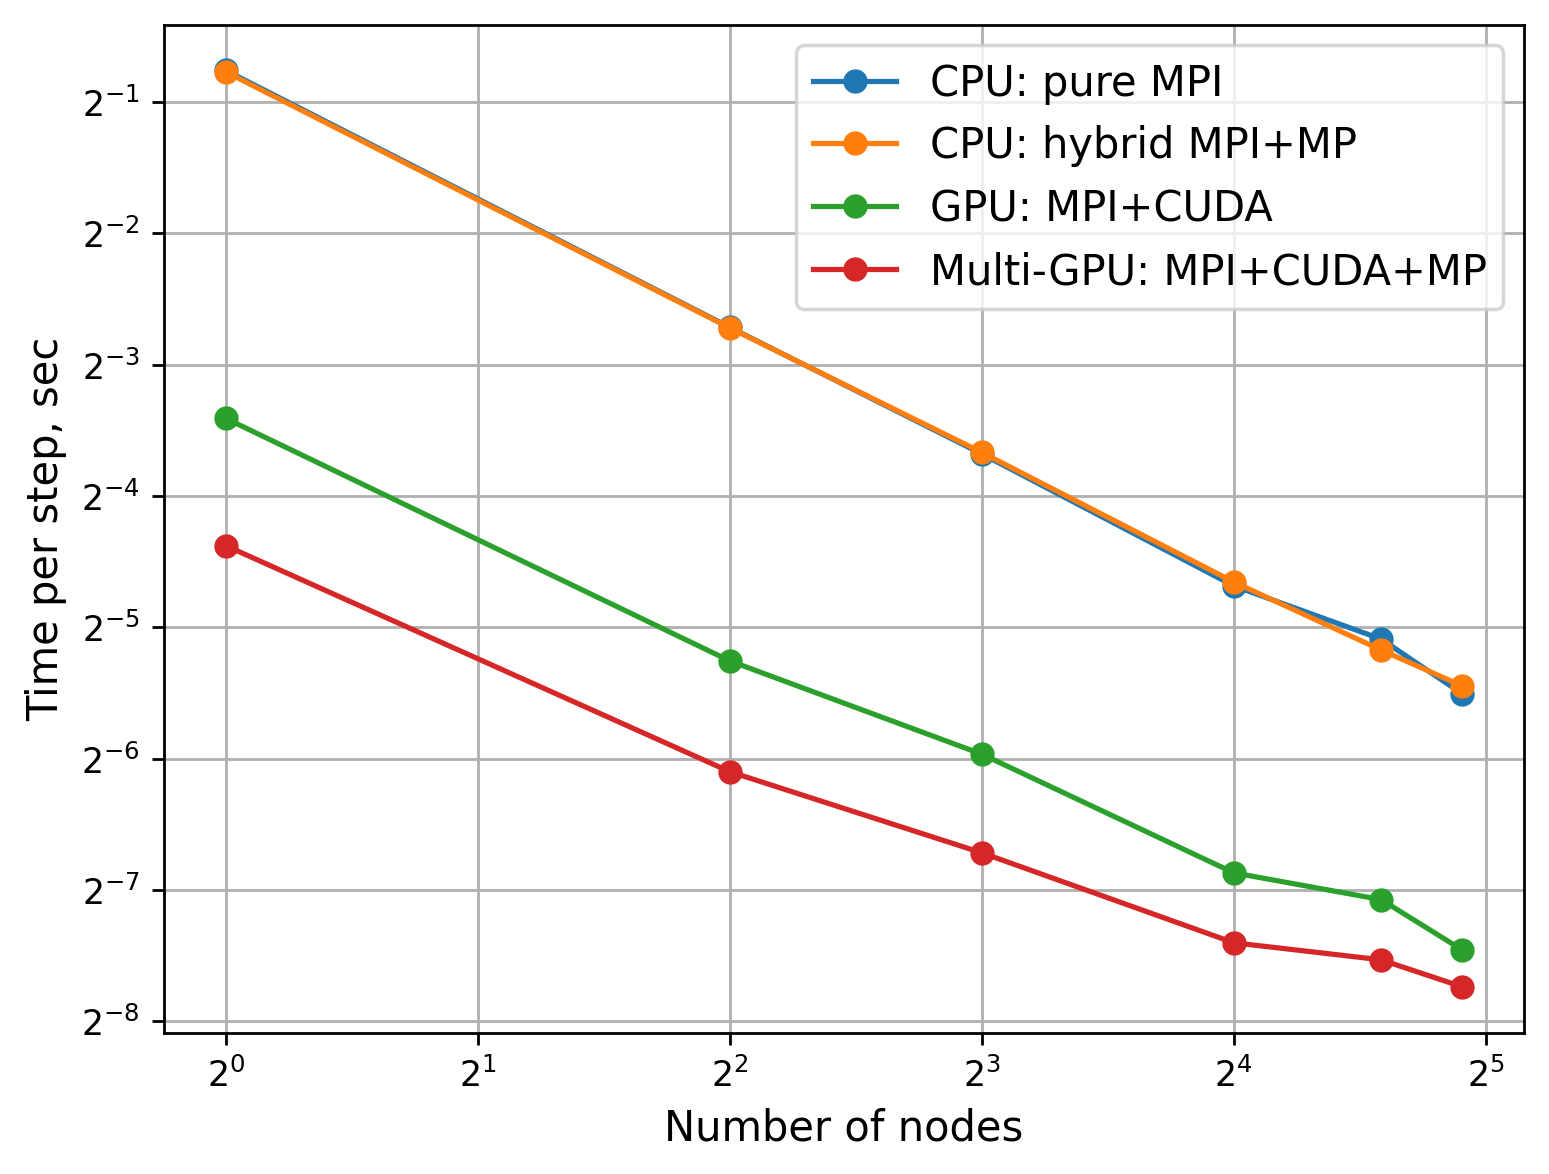
\includegraphics[width=\linewidth]{v3_3_6100x4460_pascal_time_multiGPU_V.png}
	\subcaption{Время одного шага модели (в логарифмической шкале)}
	\end{minipage}
	\vspace{3pt}
	\caption{Масштабируемость методов для расчётов мелкой воды с использованием GPU в сравнении с методами расчётов на CPU}
	\label{fig:TheBox}
\end{figure}

Было также подремонтировано, что, за счёт перекрытия вычислений с передачей данных, асинхронный подход MPI-OpenMP-CUDA лучше масштабируется до 8 узлов и на 28\% производительнее на 8 графических процессорах, чем синхронный подход без перекрытия вычислений с передачей данных. Продемонстрировано преимущество использования метода балансировки нагрузки вычислений на примере расчёта акватории Азовского моря с разрешением в 250 метров. Было показано, что производительность расчётов с балансировкой нагрузки вычислений превосходят производительность расчётов без балансировки на 30\% на 16 узлах как при использовании CPU, так и при использовании GPU.

\begin{figure}[!ht]
	\begin{minipage}{1\linewidth}
	\centering
	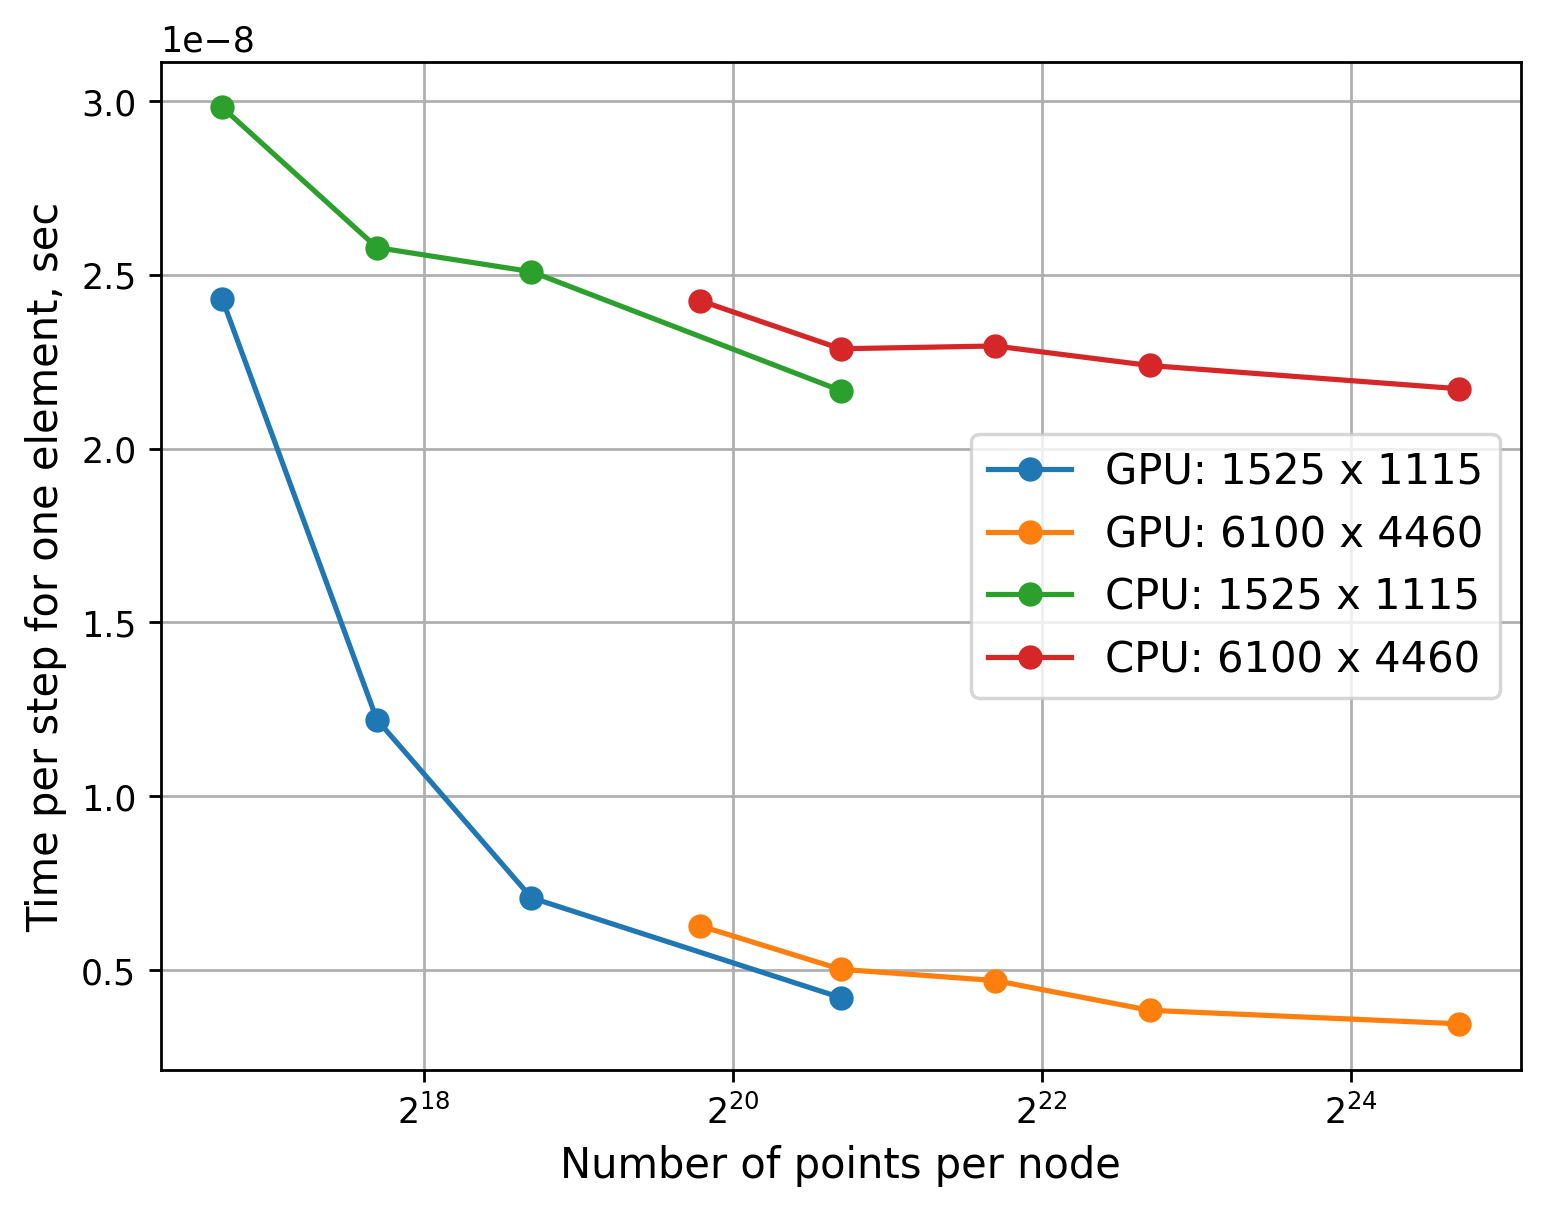
\includegraphics[width=0.5\linewidth]{v3_3_pascal_analysic_fix_1.png}
	\end{minipage}
	\vspace{3pt}
	\caption{Производительность на одну точку сетки при вычислениях на CPU и GPU}
	\label{fig:TheBox_full}
\end{figure}

В разделе продемонстрирована эффективность блочного подхода, а именно что,
выбирая малые размеры блоков, компенсируются затраты на копирование границ блоков при синхронизации за счет эффективной работа с кэш памя­тью.

	\begin{figure}[htb!]
    \begin{minipage}[h]{0.48\linewidth}
    \center{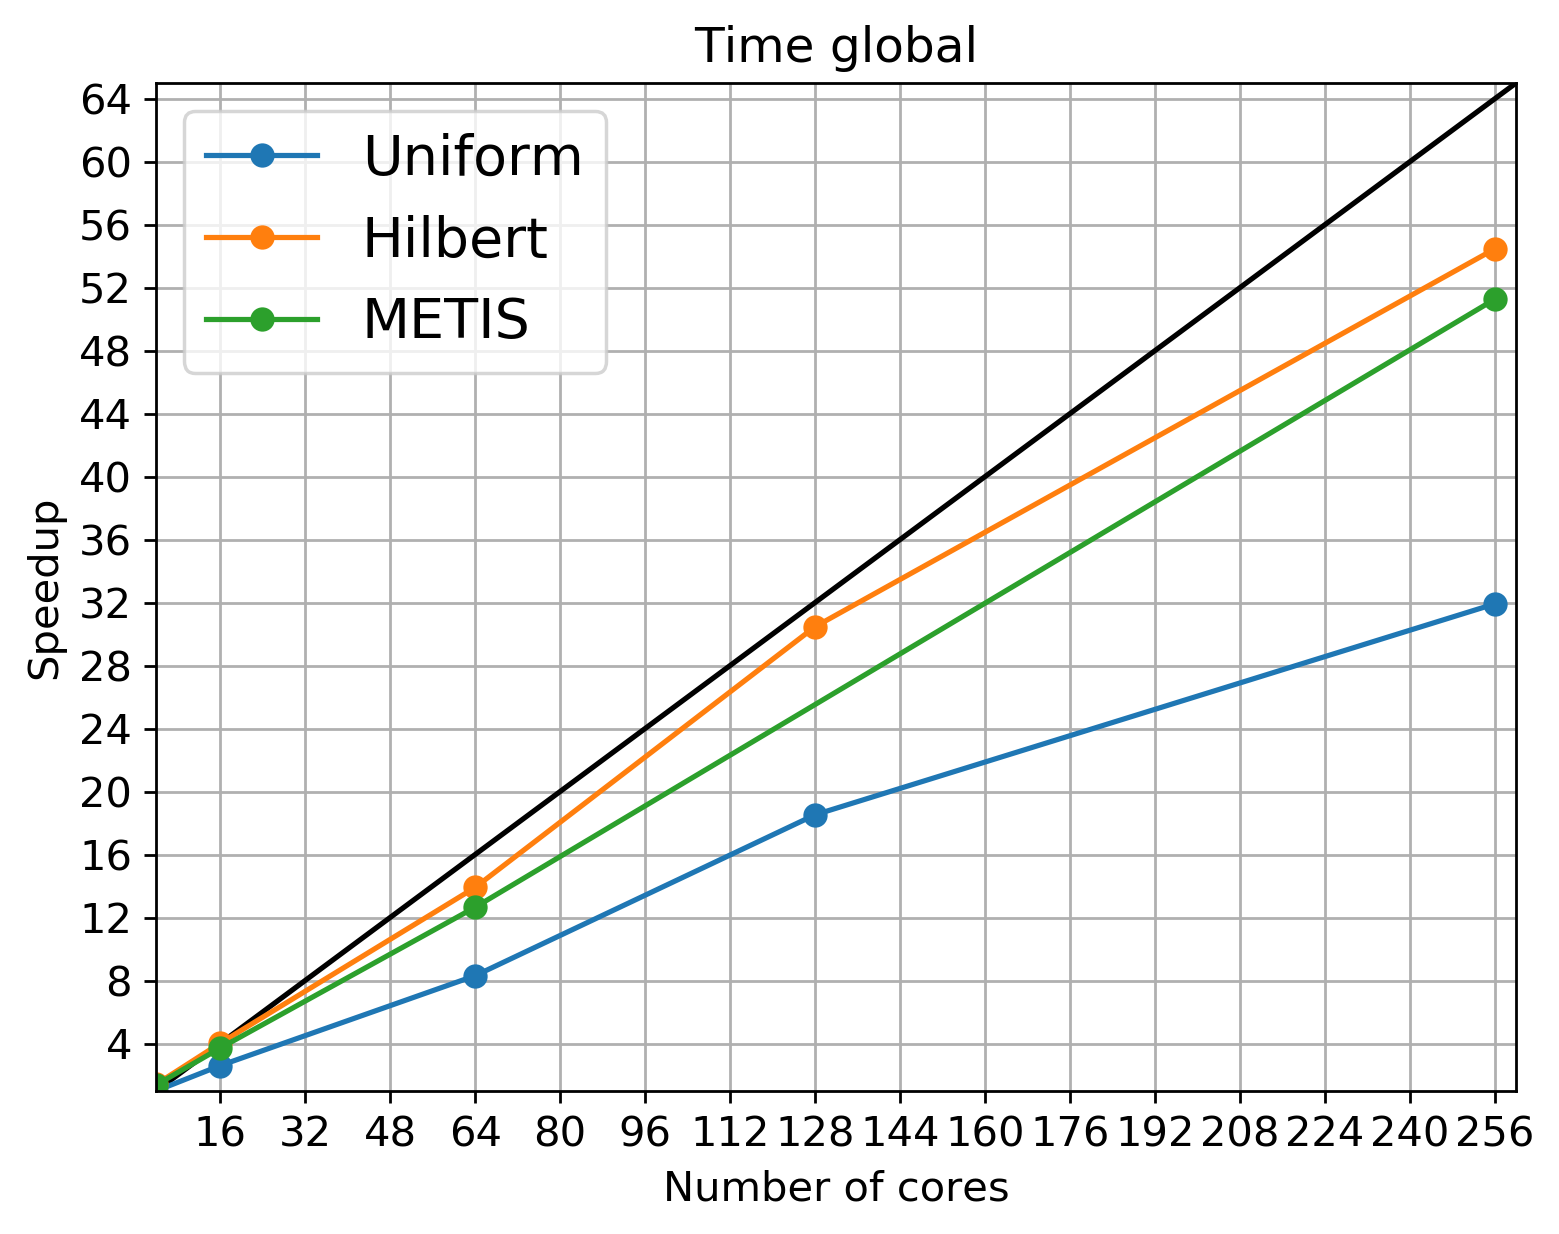
\includegraphics[width=1.0\linewidth]{plot4_upd_global.png}}
    \end{minipage}
    \hfill
    \begin{minipage}[h]{0.48\linewidth}
    \center{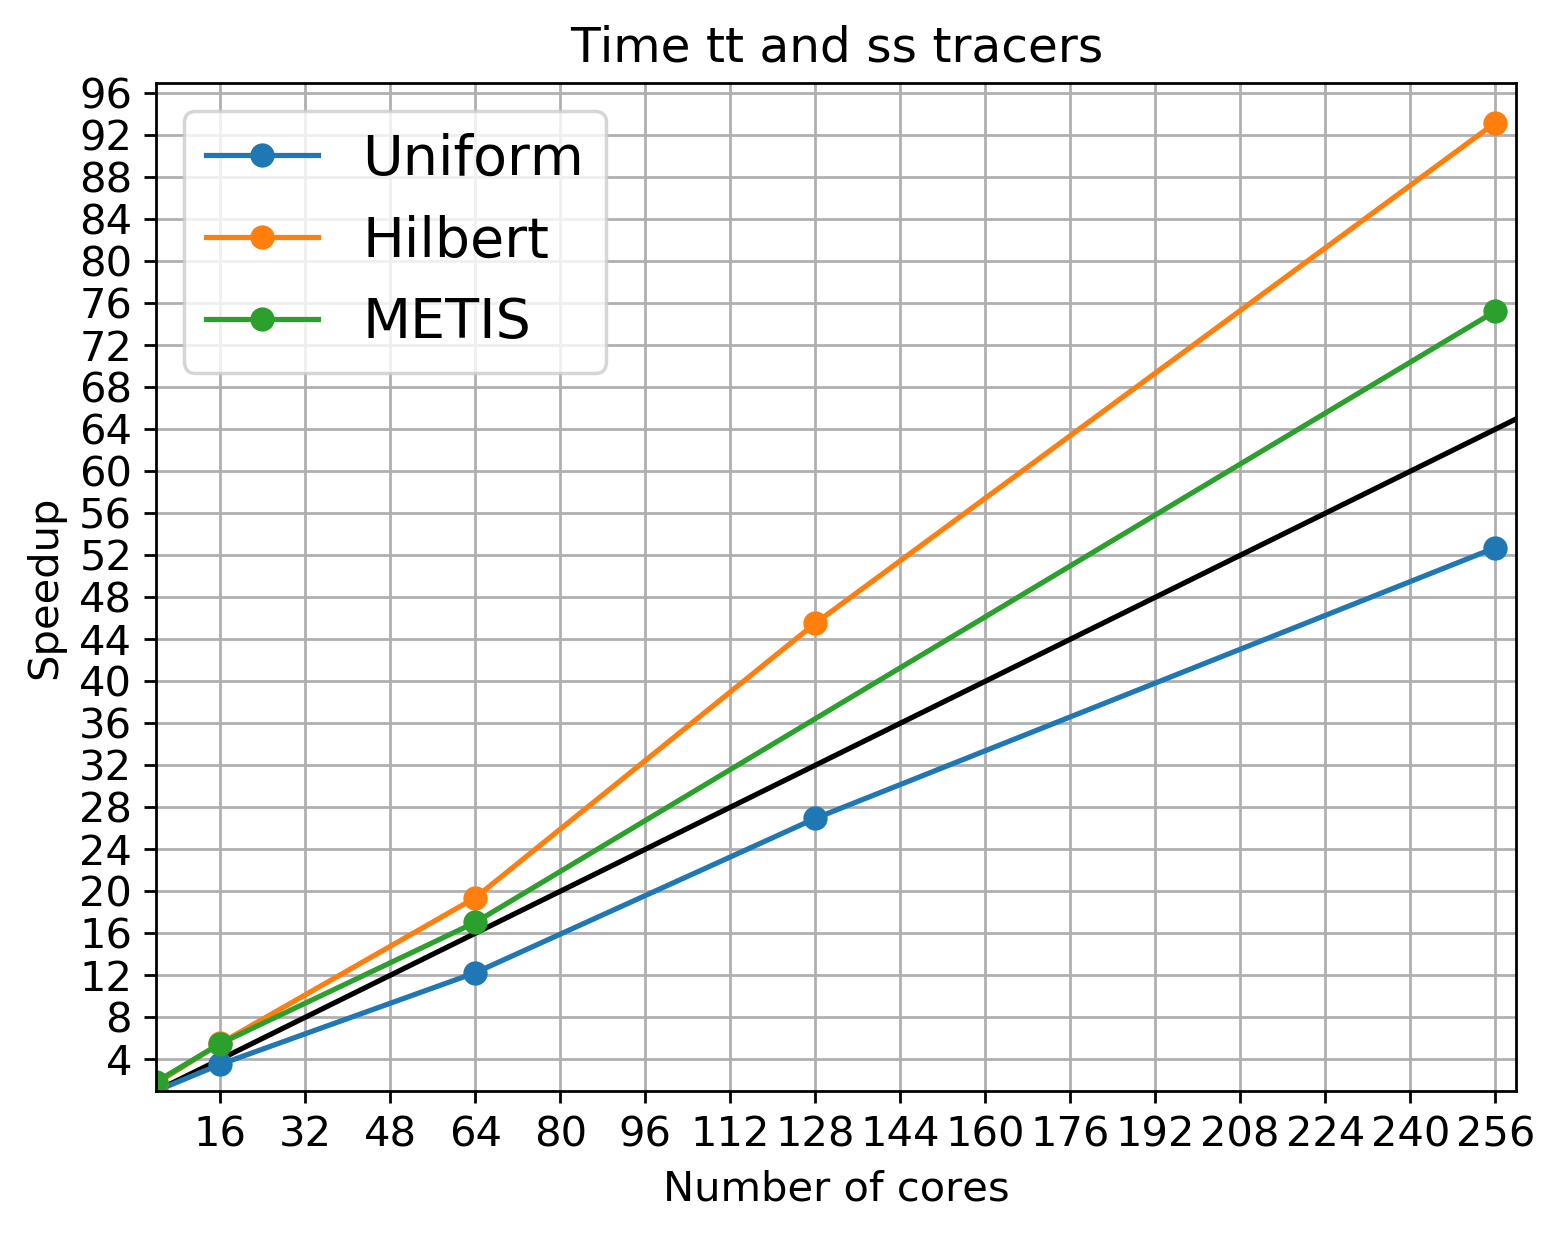
\includegraphics[width=1.0\linewidth]{plot4_upd_tt_ss.png}}
    \end{minipage}
    \caption{Модель океана INMOM. Ускорение метода разбиения с использованием кривых Гильберта в сравнении с равномерным разбиением и с METIS. 1) Общее время работы модели. 2) Расчет температуры и солености. 
    Чёрная линия соответствует линейному ускорению.}
    \label{fig:inmom_hilbert1}
    \end{figure}
    
     \begin{figure}[htb!]
    \begin{minipage}[h]{0.48\linewidth}
    \center{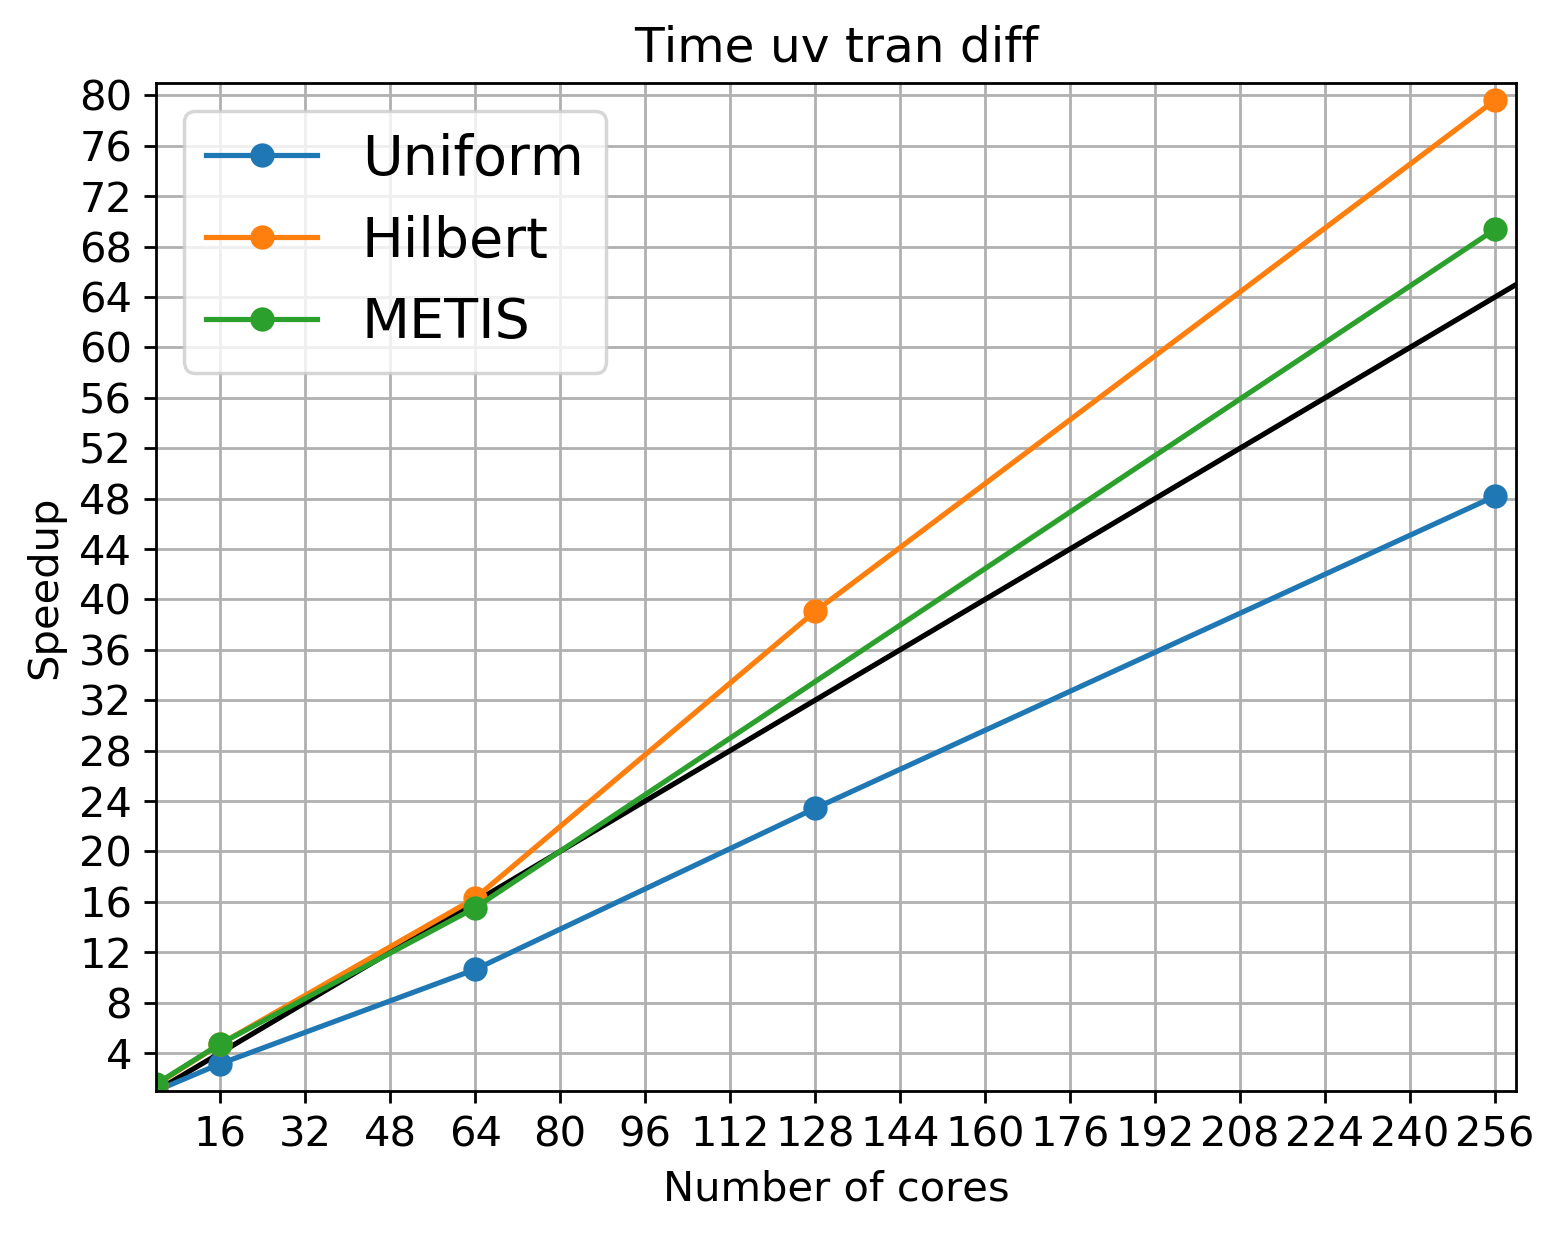
\includegraphics[width=1.0\linewidth]{plot4_upd_uv_tran_diff.png}}
    \end{minipage}
    \hfill
    \begin{minipage}[h]{0.48\linewidth}
    \center{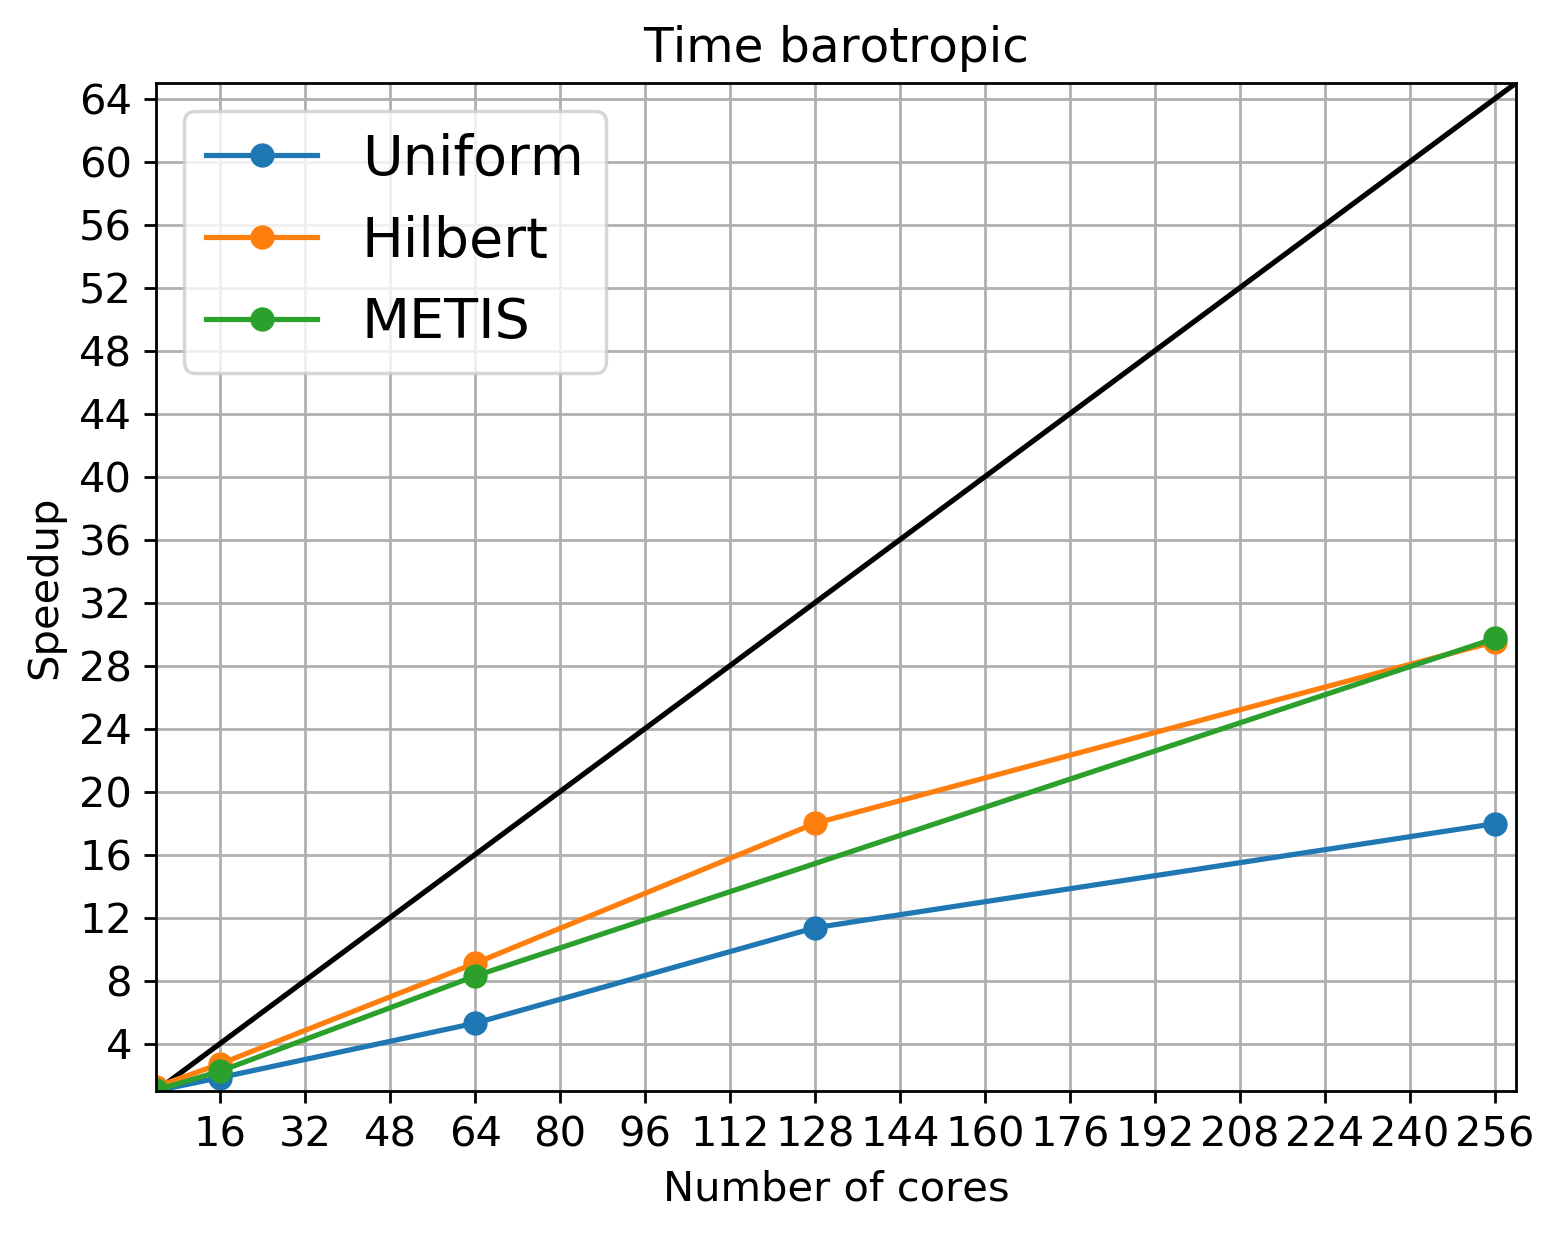
\includegraphics[width=1.0\linewidth]{plot4_upd_barotrop.png}}
    \end{minipage}
    \caption{Модель океана INMOM. Ускорение метода разбиения с использованием кривых Гильберта в сравнении с равномерным разбиением и с METIS. 1) Расчет переноса и диффузии для компонентов скорости. 2) Баротропная адаптация. 
    Чёрная линия соответствует линейному ускорению.}
    \label{fig:inmom_hilbert2}
    \end{figure}
    
В \underline{\textit{разделе 4.2}} приведены результаты исследования масштабируемости сигма-модели общей циркуляции океана INMOM.
В разделе приводятся результаты по тестированию метода нагрузки балансировки вычислений с использованием кривых Гильберта уже примени­тельно к полной трехмерной сигма-модели циркуляции океана INMOM. Тестирование модели проводилось на кластере ИВМ РАН для акватории Азовского моря.
Продемонстрировано, что методы балансировки нагрузки вычислений дают сверхлинейное ускорение для расче­тов температуры и солености и для расчета переноса и диффузии компонентов скорости, см рис. \ref{fig:inmom_hilbert1} и рис. \ref{fig:inmom_hilbert2}.
Это связано с тем, что при увеличении числа ядер, большая часть блоков, попадающих полностью на сушу, выпадает из рассмотрения. Более то­го, размер каждого блока становится мал и работа с кэш памятью становится наиболее эффективной.
Для общего расчетного времени модели метод балансировки нагрузки дает почти линейное ускорение и по сравнению с равномерным разбиением без балансировки нагрузки ускорение больше в $\sim 1.7$ раза, см. рис. \ref{fig:inmom_hilbert1}.

\FloatBarrier
\pdfbookmark{Заключение}{conclusion}                                  % Закладка pdf
В \underline{\textbf{заключении диссертации}} приведены основные результаты работы, которые заключаются в следующем:
%% Согласно ГОСТ Р 7.0.11-2011:
%% 5.3.3 В заключении диссертации излагают итоги выполненного исследования, рекомендации, перспективы дальнейшей разработки темы.
%% 9.2.3 В заключении автореферата диссертации излагают итоги данного исследования, рекомендации и перспективы дальнейшей разработки темы.
%\begin{enumerate}
%  \item На основе анализа \ldots
%  \item Численные исследования показали, что \ldots
%  \item Математическое моделирование показало \ldots
%  \item Для выполнения поставленных задач был создан \ldots
%\end{enumerate}

\begin{enumerate}
\item В работе разработана программная архитектура на принципе разделения обязанностей для модели общей циркуляции океана INMOM и, в частности,  модели мелкой воды. Разработанная программная архитектура предоставляет гибкий переход на гибридные модели параллельного программирования с использованием технологий MPI, OpenMP, CUDA.
\item На основе программной архитектуры были разработаны гибридные модели параллельного программирования для эффективного использования на массивно-параллельных многопроцессорных и гетерогенных вычислительных системах.
\item Разработан метод балансировки нагрузки вычислений на процессорах для улучшения масштабируемости и производительности моделей на высокопроизводительных вычислительных системах
\item Исследована масштабируемость и производительность предложенных методов на массивно-параллельных и гетерогенных вычислительных системах.
\end{enumerate}

\pdfbookmark{Литература}{bibliography}                                % Закладка pdf

%При использовании пакета \verb!biblatex! список публикаций автора по теме
%диссертации формируется в разделе <<\publications>>\ файла
%\verb!common/characteristic.tex!  при помощи команды \verb!\nocite!

\ifdefmacro{\microtypesetup}{\microtypesetup{protrusion=false}}{} % не рекомендуется применять пакет микротипографики к автоматически генерируемому списку литературы
\urlstyle{rm}                               % ссылки URL обычным шрифтом
\ifnumequal{\value{bibliosel}}{0}{% Встроенная реализация с загрузкой файла через движок bibtex8
    \renewcommand{\bibname}{\large \bibtitleauthor}
    \nocite{*}
    \insertbiblioauthor           % Подключаем Bib-базы
    %\insertbiblioexternal   % !!! bibtex не умеет работать с несколькими библиографиями !!!
}{% Реализация пакетом biblatex через движок biber
    % Цитирования.
    %  * Порядок перечисления определяет порядок в библиографии (только внутри подраздела, если `\insertbiblioauthorgrouped`).
    %  * Если не соблюдать порядок "как для \printbibliography", нумерация в `\insertbiblioauthor` будет кривой.
    %  * Если цитировать каждый источник отдельной командой --- найти некоторые ошибки будет проще.
    %
    %% authorvak
    \nocite{vakbib1}%
    \nocite{vakbib2}%
    %
    %% authorwos
    \nocite{wosbib1}%
    %
    %% authorscopus
    \nocite{scbib1}%
    %
    %% authorpathent
    \nocite{patbib1}%
    %
    %% authorprogram
    \nocite{progbib1}%
    %
    %% authorconf
    \nocite{confbib1}%
    \nocite{confbib2}%
    %
    %% authorother
    \nocite{bib1}%
    \nocite{bib2}%

    \ifnumgreater{\value{usefootcite}}{0}{
        \begin{refcontext}[labelprefix={}]
            \ifnum \value{bibgrouped}>0
                \insertbiblioauthorgrouped    % Вывод всех работ автора, сгруппированных по источникам
            \else
                \insertbiblioauthor      % Вывод всех работ автора
            \fi
        \end{refcontext}
    }{
        \ifnum \totvalue{citeexternal}>0
            \begin{refcontext}[labelprefix=A]
                \ifnum \value{bibgrouped}>0
                    \insertbiblioauthorgrouped    % Вывод всех работ автора, сгруппированных по источникам
                \else
                    \insertbiblioauthor      % Вывод всех работ автора
                \fi
            \end{refcontext}
        \else
            \ifnum \value{bibgrouped}>0
                \insertbiblioauthorgrouped    % Вывод всех работ автора, сгруппированных по источникам
            \else
                \insertbiblioauthor      % Вывод всех работ автора
            \fi
        \fi
        %  \insertbiblioauthorimportant  % Вывод наиболее значимых работ автора (определяется в файле characteristic во второй section)
        \begin{refcontext}[labelprefix={}]
            \insertbiblioexternal            % Вывод списка литературы, на которую ссылались в тексте автореферата
        \end{refcontext}
        % Невидимый библиографический список для подсчёта количества внешних публикаций
        % Используется, чтобы убрать приставку "А" у работ автора, если в автореферате нет
        % цитирований внешних источников.
        \printbibliography[heading=nobibheading, section=0, env=countexternal, keyword=biblioexternal, resetnumbers=true]%
    }
}
\ifdefmacro{\microtypesetup}{\microtypesetup{protrusion=true}}{}
\urlstyle{tt}                               % возвращаем установки шрифта ссылок URL
